\documentclass[]{beamer}

\mode<presentation>
{
  \usetheme{Warsaw}
  % or ...

  \setbeamercovered{transparent}
  % or whatever (possibly just delete it)
}

\usepackage{xunicode}
\usepackage[slantfont,boldfont]{xeCJK}
\usepackage{ulem}

\setCJKmainfont{AR PL UKai CN}

\XeTeXlinebreaklocale "zh"
\XeTeXlinebreakskip = 0pt plus 1pt


\graphicspath{{./software_process/}}

\title[Thinking in SE]
{软件过程}

\subtitle
{软件工程导论之六} % (optional)

\author[\url{http://sunner.cn}] % (optional, use only with lots of authors)
{王宇颖 \and 孙志岗}
% - Use the \inst{?} command only if the authors have different
%   affiliation.

\institute[哈尔滨工业大学] % (optional, but mostly needed)
{
  计算机科学与技术学院\\
  哈尔滨工业大学}
% - Use the \inst command only if there are several affiliations.
% - Keep it simple, no one is interested in your street address.

\date[Short Occasion] % (optional)
{2011-10-14/17}

\subject{Slides}
% This is only inserted into the PDF information catalog. Can be left
% out. 



% If you have a file called "university-logo-filename.xxx", where xxx
% is a graphic format that can be processed by latex or pdflatex,
% resp., then you can add a logo as follows:

% \pgfdeclareimage[height=0.5cm]{university-logo}{university-logo-filename}
% \logo{\pgfuseimage{university-logo}}


% Delete this, if you do not want the table of contents to pop up at
% the beginning of each subsection:
\AtBeginSubsection[]
{
  \begin{frame}<beamer>{主要内容}
    \tableofcontents[currentsection,currentsubsection]
  \end{frame}
}

% \beamerdefaultoverlayspecification{<+->}

\begin{document}

\begin{frame}
  \titlepage
\end{frame}

\begin{frame}{主要内容}
  \tableofcontents
  % You might wish to add the option [pausesections]
\end{frame}

\section{软件生命周期}

\begin{frame}
  \begin{columns}
    \begin{column}{.5\textwidth}
      软件的一生包含五个过程:
      \begin{itemize}
        \item 需求分析
        \item 系统设计
        \item 编码开发
        \item 软件测试
        \item 部署和维护
      \end{itemize}
    \end{column}
    \begin{column}{.5\textwidth}
      \only<2>{
        \begin{block}{}
          这是相当\alert{坎坷}的一生\dots

          \begin{center}
            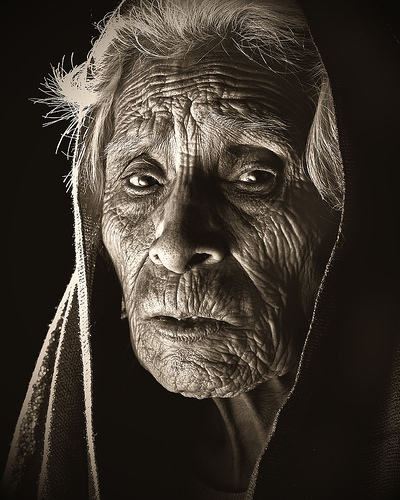
\includegraphics[width=4cm]{hardlife}
          \end{center}
        \end{block}
      }
    \end{column}
  \end{columns}
\end{frame}

\begin{frame}{软件的悲催生活}
  \begin{columns}
    \begin{column}{.2\paperwidth}
      \begin{center}
        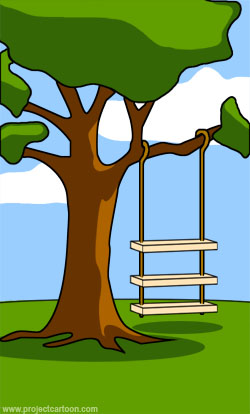
\includegraphics[width=2cm]{prj_user}

        \scriptsize 用户如此描述需求
      \end{center}
    \end{column}
    \only<2->{
    \begin{column}{.2\paperwidth}
      \begin{center}
        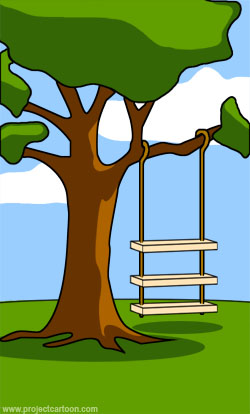
\includegraphics[width=2cm]{prj_user}

        \scriptsize 用户如此描述需求
      \end{center}
    \end{column}}
    \only<3->{
    \begin{column}{.2\paperwidth}
      \begin{center}
        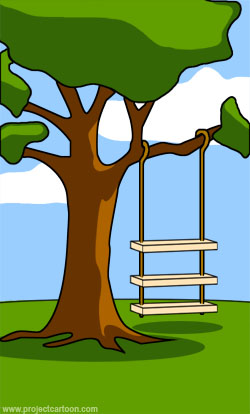
\includegraphics[width=2cm]{prj_user}

        \scriptsize 用户如此描述需求
      \end{center}
    \end{column}}
    \only<4->{
    \begin{column}{.2\paperwidth}
      \begin{center}
        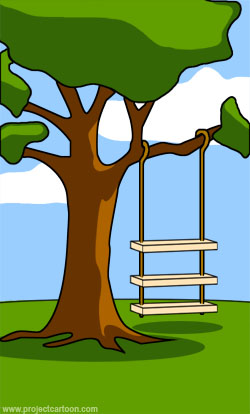
\includegraphics[width=2cm]{prj_user}

        \scriptsize 用户如此描述需求
      \end{center}
    \end{column}}
    \only<5->{
    \begin{column}{.2\paperwidth}
      \begin{center}
        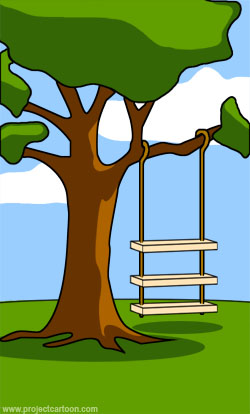
\includegraphics[width=2cm]{prj_user}

        \scriptsize 用户如此描述需求
      \end{center}
    \end{column}}
  \end{columns}
\end{frame}

\section{需求分析}

\section{系统设计}

\section{编码开发}

\section{软件测试}

\section{部署和维护}

\end{document}
